% Chapter Template

\chapter{Marco Teórico} % Main chapter title

\label{Chapter2} % Change X to a consecutive number; for referencing this chapter elsewhere, use \ref{ChapterX}

\lhead{Capítulo 2. \emph{Marco Teórico}} % Change X to a consecutive number; this is for the header on each page - perhaps a shortened title

\section{Cerramientos Eléctricos}
Cuando hablamos de cerramientos eléctricos se hacer referencia a todos los dispositivos
de funcionamiento electromecánico destinados a ofrecer la función de cerradura para aperturas de instalaciones domiciliarias, comerciales e industriales.
Se listan a continuación ejemplos de estos dispositivos.
\begin{itemize}
	\item Cerraduras por electro-imán.
	\item Cerraduras de perno.
	\item Portones automatizados.
	\item Barreras automáticas.
	\item Pasadores eléctricos.
	\item Traba-pestillo eléctrico.
	\item Pestillo eléctrico para cajones o guarda equipajes.
	\item Puertas de Ascensor con control de acceso.
\end{itemize}


\subsection{Principio de Funcionamiento}
Aunque todos los cerramientos eléctricos comparten la misma funcionalidad existe una variedad acotada de principios de funcionamiento, diseño industrial o factor de forma entre los cuales podemos mencionar:
\begin{itemize}
	\item Solenoide y Perno
	\item Solenoide y Clavija
	\item Electroimán
	\item Motor Eléctrico
\end{itemize}

\subsubsection{Solenoide y Perno}
Un solenoide es enrollado alrededor de un eje cilíndrico dieléctrico hueco que a su vez envuelve un perno también cilíndrico pero metálico. Este solenoide está conectado en un circuito de corriente continua. Cuando se alimenta dicho circuito el campo magnético inducido en el núcleo del solenoide genera corrientes de Foucault sobre el perno que es desplazado por la fuerza del campo magnético, generando así la acción de traba o bloqueo sobre el herraje de la abertura. 
Este tipo de principio de funcionamiento es el que emplean dispositivos tales como los pestillos eléctricos y las cerraduras de perno que se muestran en la figura ~\ref{fig:sol+perno}.

\begin{figure}[htbp]
	\centering
	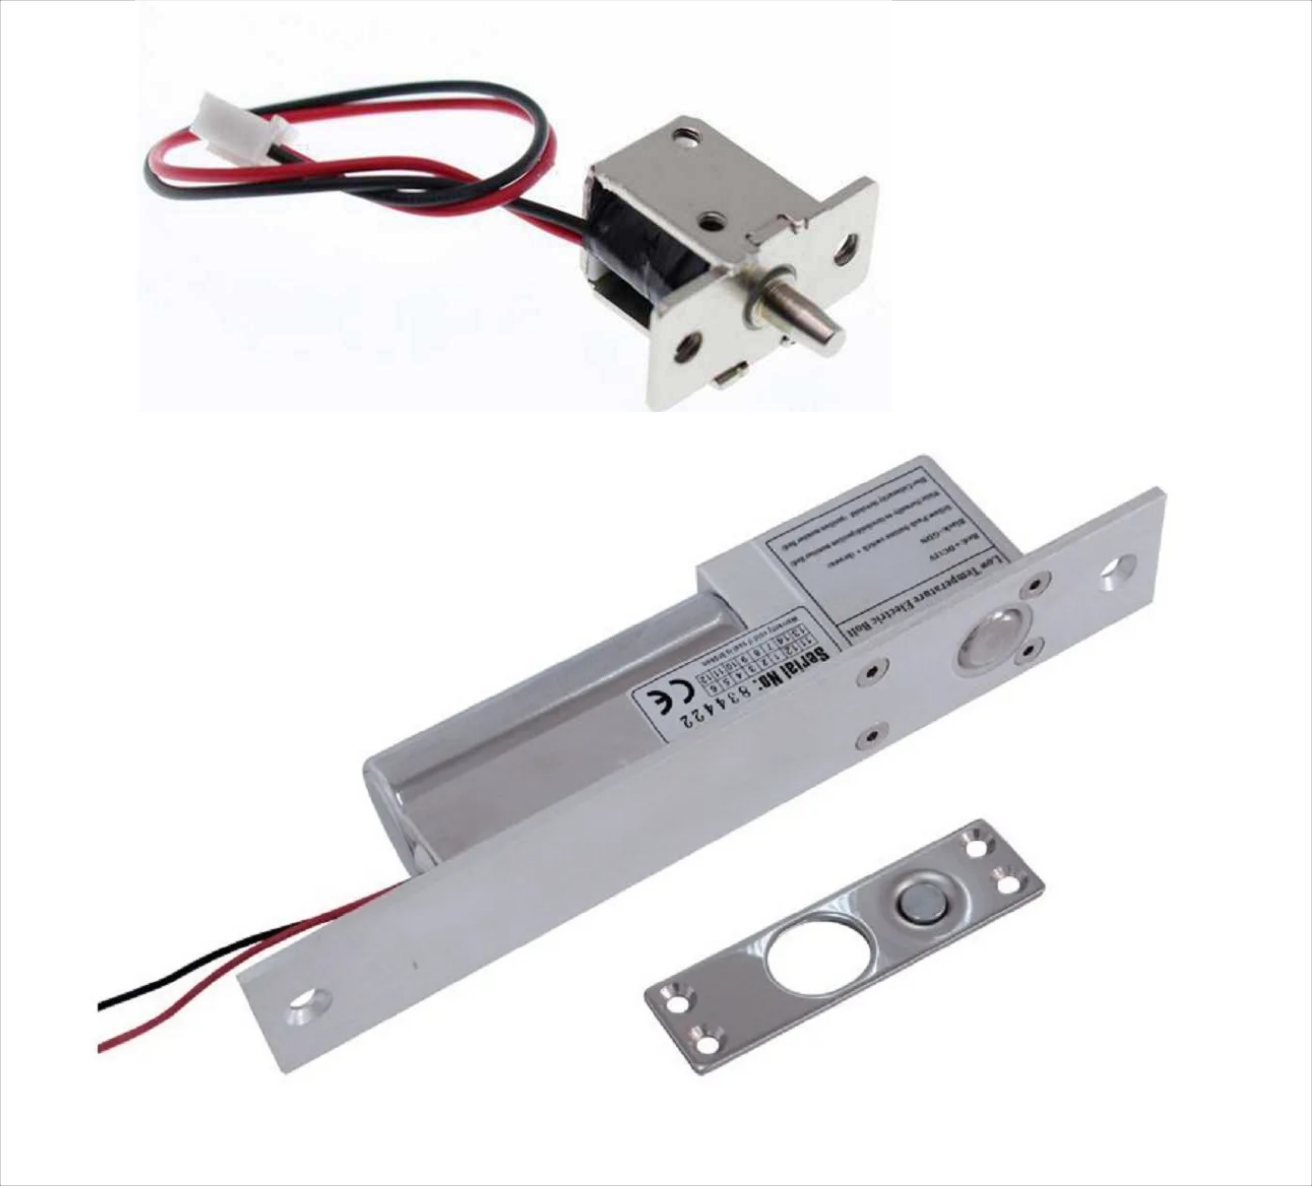
\includegraphics[width=0.5\textwidth]{Pictures/sol+perno.png}
	\rule{35em}{1pt}
	\caption[Cerramientos de perno]{Se muestran ejemplos de cerramientos eléctricos que funcionan con solenoide y perno. }
	\label{fig:sol+perno}
\end{figure}

\subsubsection{Solenoide y Clavija}
De una forma similar a la descripta para el caso del perno, un solenoide se utiliza para formar un pequeño electroimán en el interior del dispositivo. La fuerza inducida deforma de manera elástica una clavija o chapa metálica delgada en forma de ele. Esta deformación libera el mecanismo que bloquea el movimiento del pestillo. Este es el caso del traba-pestillo eléctrico o del pasador eléctrico cuyos ejemplos se muestran en la figura ~\ref{fig:sol+clav}.

\begin{figure}[htbp]
	\centering
	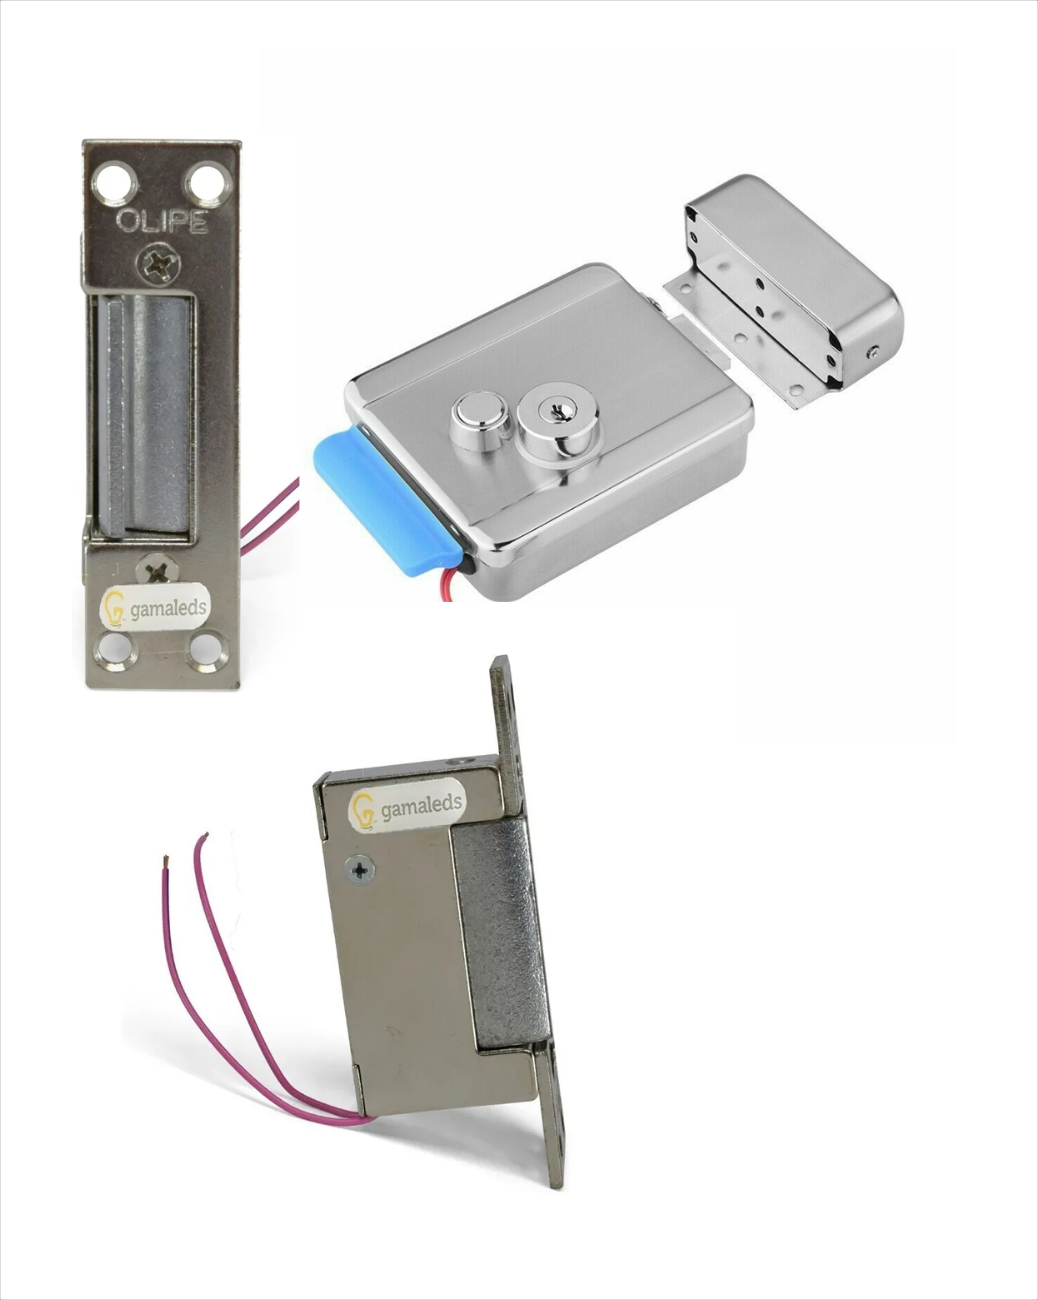
\includegraphics[width=0.35\textwidth]{Pictures/sol+clav.png}
	\rule{35em}{1pt}
	\caption[Cerramientos de perno]{Se muestran ejemplos de cerramientos eléctricos que funcionan con solenoide y clavija. }
	\label{fig:sol+clav}
\end{figure}

\subsubsection{Electroimán}
En esta forma de funcionamiento se construye un electroimán de dimensiones considerables capaz de ejercer una fuerza de atracción magnética cercana a los 300 kgF sobre una chapa metálica que también se incluye como parte del cerramiento. Por lo general incluyen en su circuito una etapa de compensación de factor de potencia para remanencia cero.
Este es el caso de la cerradura por electroimán que se muestra en la figura ~\ref{fig:cerr-mag}.

\begin{figure}[htbp]
	\centering
	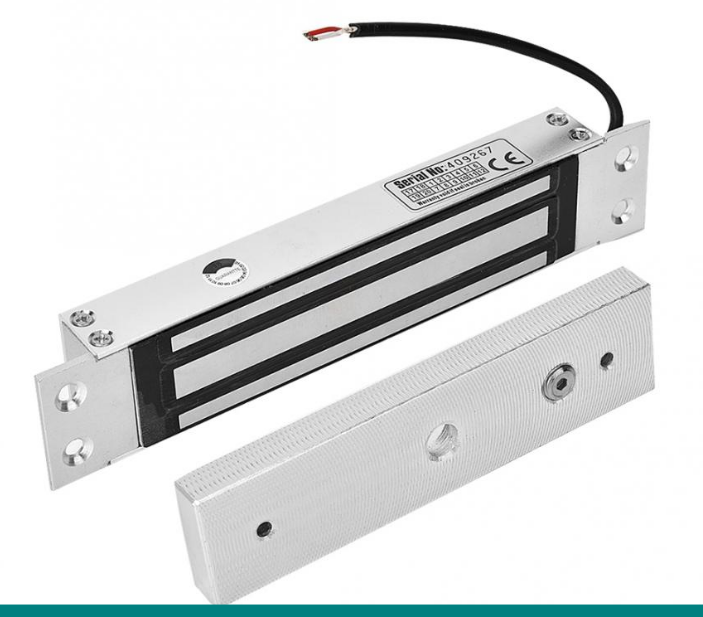
\includegraphics[width=0.4\textwidth]{Pictures/magnet.png}
	\rule{35em}{1pt}
	\caption[Cerradura Electroimán]{Se muestran un ejemplo de cerradura eléctrica que funcionan por electroimán. }
	\label{fig:cerr-mag}
\end{figure}

\subsubsection{Motor Eléctrico}
Para el caso de grandes portones de garage o acceso vehicular se utilizan motores de corriente alterna o brushless de corriente contínua con su respectivos controladores. Estos motores interactúan mecánicamente con otras interfaces mecánicas instaladas en las aperturas para posibilitar la tarea de apertura o cierre. Adicionalmente es necesario la incorporación de sensores que indiquen el estado del sistema y aseguran su correcto funcionamiento.
Todos los tipos de automatización de portones así como los sistemas de apertura con cortinas metálicas comparten el mismo principio de funcionamiento y utilizan motores similares al que se muestra en la figura ~\ref{fig:motorport}.

\begin{figure}[htbp]
	\centering
	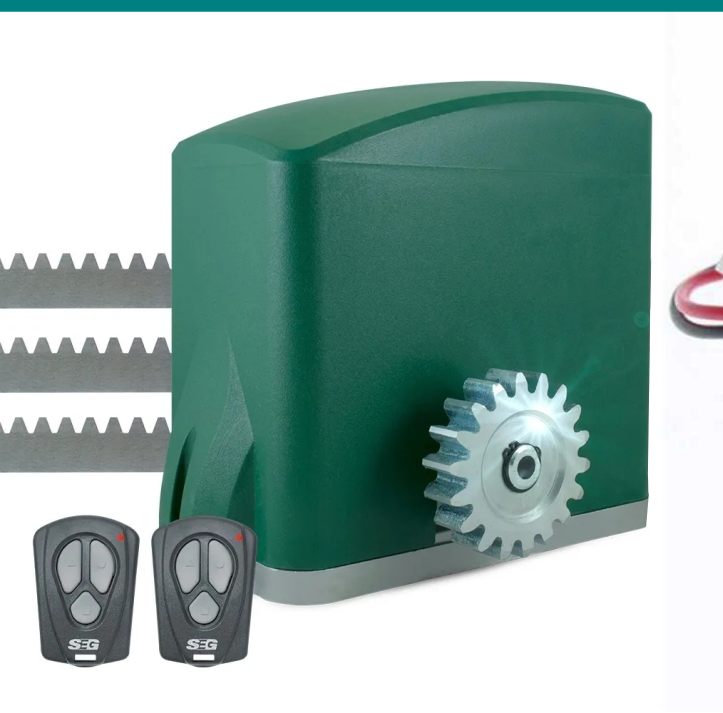
\includegraphics[width=0.4\textwidth]{Pictures/motor.png}
	\rule{35em}{1pt}
	\caption[Motor Portones Automatizados]{Motor empleado en sistemas de automatización de portones de garaje o accesos vehiculares. }
	\label{fig:motorport}
\end{figure}

\section{Controladores}
Todos los cerramientos eléctricos mencionados anteriormente no funcionan por si mismos sino que requieren de un dispositivo controlador.
Algunos ejemplos se muestran en la figura ~\ref{fig:controladoresacceso}.\\
\begin{figure}[htbp]
	\centering
	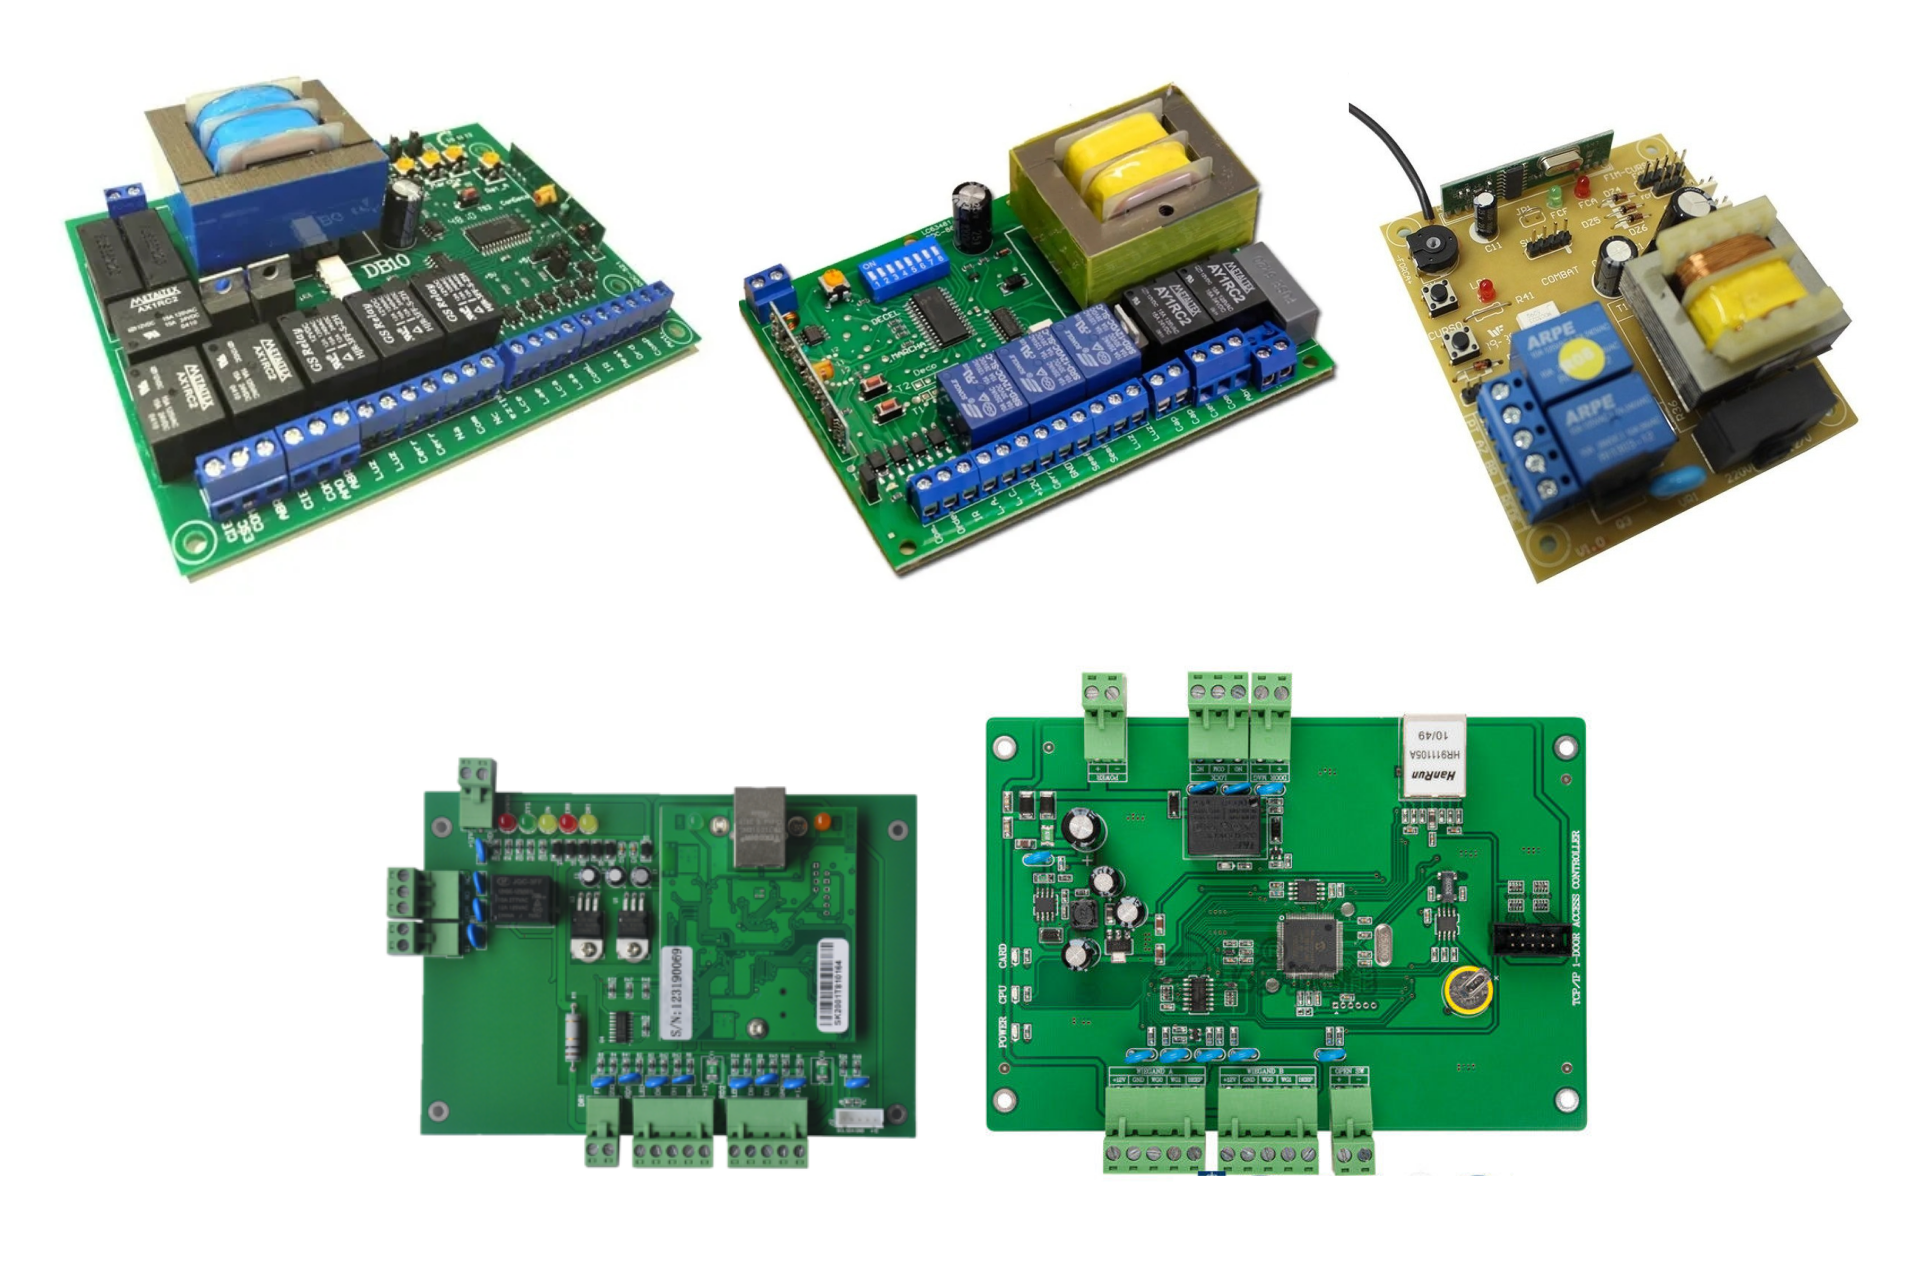
\includegraphics[width=0.8\textwidth]{Pictures/controladoresacceso.png}
	\rule{35em}{1pt}
	\caption[Controladores de Acceso]{Algunos ejemplos de controladores de cerramientos eléctricos.}
	\label{fig:controladoresacceso}
\end{figure}
Estos controladores son circuitos electrónicos que se encargan de generar las señales de activación y/o control de los cerramientos eléctricos. El usuario podrá actuar sobre el cerramiento eléctrico a través de diversos modos de accionamiento, se mencionan los más habituales:
\begin{itemize}
	\item Portero telefónico
	\item Contraseña por teclado
	\item Lector biométrico
	\item Llave electrónica
	\item Botón externo
\end{itemize}

Para dar soporte a una o múltiples formas de accionamiento el controlador ofrece una interfaz de configuración y los componentes necesarios para su operación.
En el caso de los cerramientos a motor es necesario incluir sensores de apertura y funcionamiento.

\subsection{Sensores}
Por lo general solo son empleados por los controladores para cerramientos a motor. Existen vario tipos de sensores para estos controladores se mencionan los más utilizados:
\begin{itemize}
	\item Sensores de Fin de Carrera
	\item Encoder Digital
\end{itemize}
. 
\subsubsection{Sensores de Fin de Carrera}
\label{section:fincarrera}
Se utiliza el plural para este caso de sensado porque se utilizan de a pares. Se trata de un par de sensores binarios que indican apertura o cierre total del cerramiento.
Suelen venir en dos presentaciones con modo de funcionamiento distinto.\\
\textbf{Por proximidad magnética:} En este caso cada uno de los sensores está compuesto por un imán permanente y un switch encapsulado como se muestra en la figura ~\ref{fig:fincarrera}(a). Este encapsulado contiene en su interior un filamento de material ferromagnético flexible que al aproximarse lo suficiente al imán se desplaza y cierra el circuito.\\
\textbf{Por choque mecánico:} Estos sensores son switches mecánicos muy sensibles que se instalan en los límites del marco de la abertura y al mínimo contacto con la parte móvil cierran sus circuitos. En la figura ~\ref{fig:fincarrera}(b) se muestran ejemplos de estos dispositivos.

\begin{figure}[htbp]
	\centering
	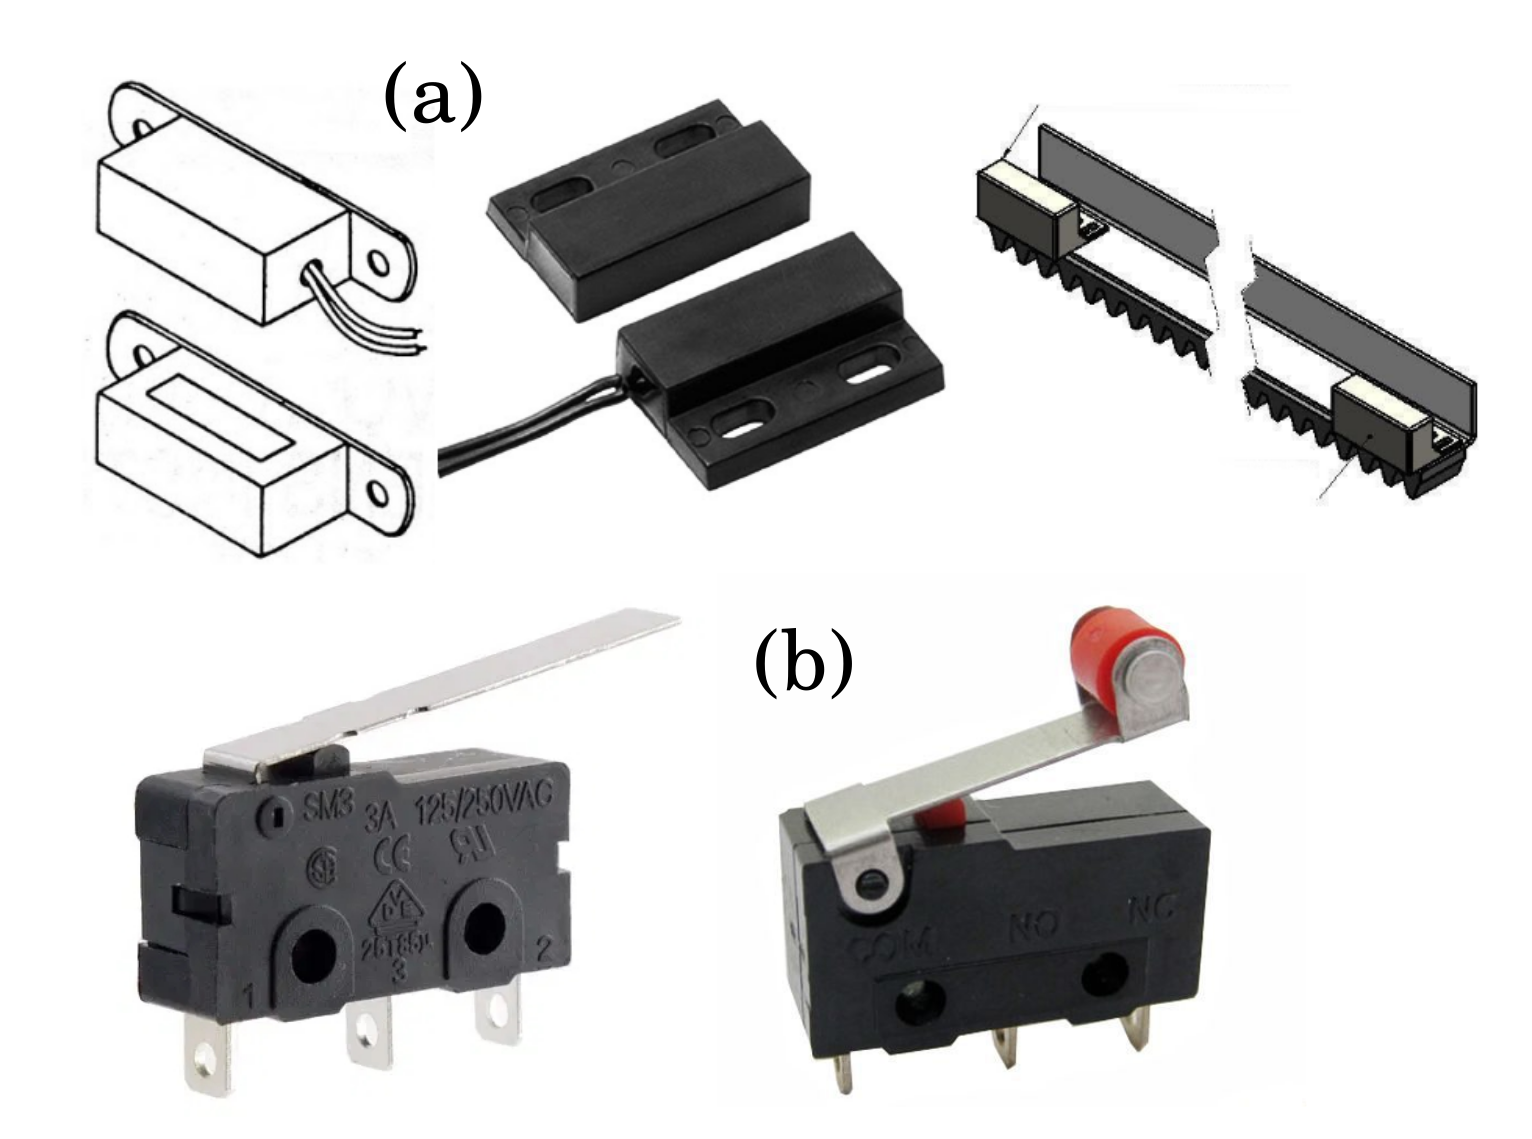
\includegraphics[width=0.6\textwidth]{Pictures/fincarrera.png}
	\rule{35em}{1pt}
	\caption[Sensores de fin de carrera]{Ejemplos de sensores de fin de carrera.(a) Sensores por proximidad magnética, (b) Sensores por choque mecánico. }
	\label{fig:fincarrera}
\end{figure}

\subsubsection{Encoder Rotativo}
Un encoder es un sensor de movimiento mecánico que genera señales digitales en respuesta al movimiento y puede proveer  información sobre la posición, la velocidad y la dirección del movimiento. En particular el econder rotativo responde al movimiento de rotación de un eje. Por lo general los controladores de cerramientos eléctricos a motor utilizan encoders rotativos incrementales que generan un tren de pulsos que se puede utilizar para determinar la posición y la velocidad del eje del motor. En la figura ~\ref{fig:encoder00} se observa la forma del tren de pulsos que genera el encoder.

\begin{figure}[htbp]
	\centering
	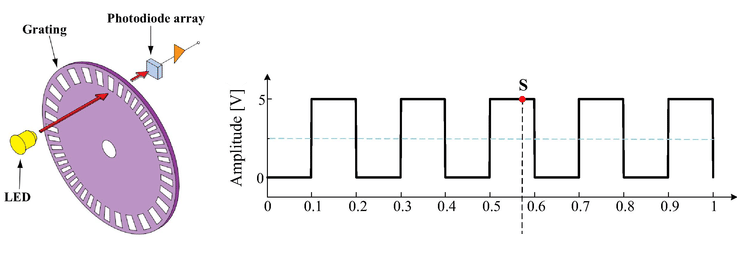
\includegraphics[width=0.8\textwidth]{Pictures/encoder00.png}
	\rule{35em}{1pt}
	\caption[Encoder Rotativo]{Ilustración simplificada de un encoder rotativo con salida de onda cuadrada TTL. }
	\label{fig:encoder00}
\end{figure}


\subsection{Monitoreo y Alerta}
La mayoría de los controladores poseen interfaces que permiten la conexión local de luminarias testigo, así como bocinas de alerta. Algunos modelos incluyen un puerto serie (RJ45, RJ14) capaz de comunicarse mediante comandos estándar con los tradicionales sistemas de alarma.

\subsubsection{Monitoreo Remoto}
Al momento de iniciar el presente proyecto integrador no existían controladoras de acceso con la funcionalidad de monitoreo remoto incorporada de fábrica.
La alternativa para tener información del cerramiento eléctrico y el estado de la abertura que opera consiste en instalar un sensor de apertura y conectarlo a una central de alarma. Estos sensores son baratos y su principio de funcionamiento coincide con el descripto para los sensores de fin de carrera y que se puede consultar en la sección ~\ref{section:fincarrera}.
Las centrales de alarma suelen estar conectadas por cableado telefónico a un servicio de monitoreo que lanza las notificaciones pertinentes según se hayan configurado.
Una basta mayoría de proveedoras de servicio de monitoreo de alarmas ahora ofrecen plataformas web o aplicaciones móviles que permiten el monitoreo de las centrales en tiempo real.

\subsection{Llaves Electrónicas y Control Remoto}
Actualmente la mayoría de los controladores de acceso soportan algún tipo de llave electrónica.
Una llave electrónica es un dispositivo electrónico que le permite al usuario operar el cerramiento eléctrico. Existen diversos tipos de llaves electrónicas a continuación se mencionan las más utilizadas.
\begin{itemize}
	\item Llaves RFID
	\item Control Remoto RF
\end{itemize}

\subsubsection{Llaves RFID}
RFID (Radio-frequency identification) es un sistema de almacenamiento y recuperación de datos a distancias cortas por emisión de radiofrecuencia de baja potencia. 
Una etiqueta RFID consiste en un pequeño circuito receptor y transmisor de radio. Cuando es activada por un pulso de interrogación electromagnético emitido por un dispositivo lector RFID cercano, la etiqueta transmite datos digitales de vuelta al lector, generalmente un número identificador.
Estas etiquetas o circuitos RFID son tan diminutos que pueden incluirse en objetos de tamaño reducido como llaveros y tarjetas, algunos ejemplos se muestran en la figura ~\ref{fig:llavesrfid}.
El usuario del sistema de acceso aproximará esta llave al lector RFID incluido en el controlador y se producirá el intercambio del número identificatorio. En caso de que ese dato esté registrado en el controlador el usuario podrá controlar el cerramiento eléctrico.

\begin{figure}[htbp]
	\centering
	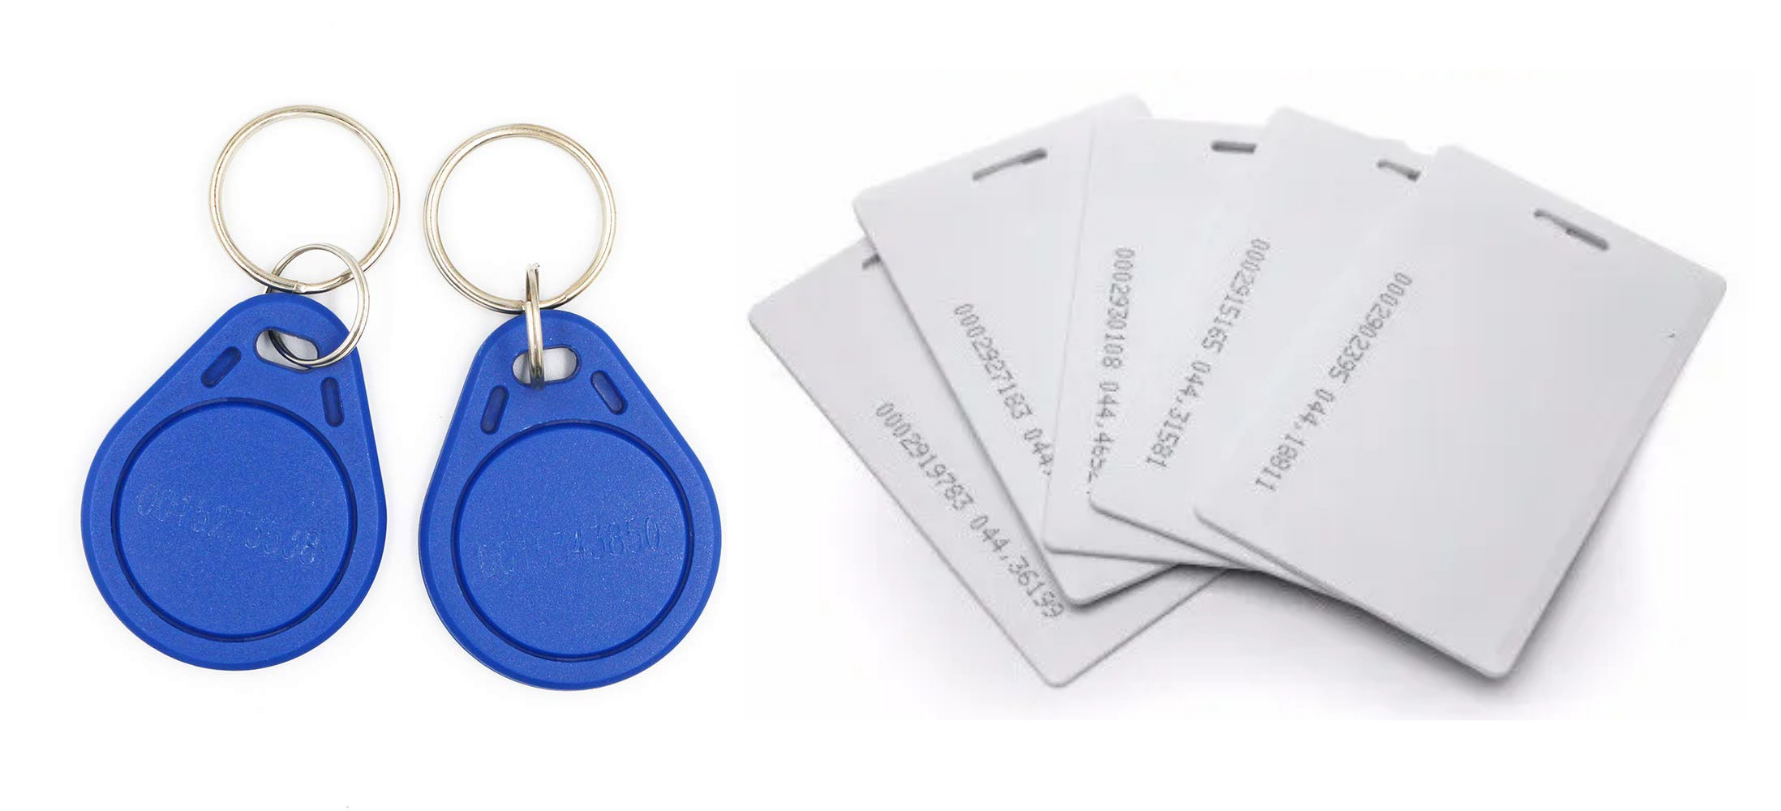
\includegraphics[width=0.8\textwidth]{Pictures/llavesrfid.png}
	\rule{35em}{1pt}
	\caption[Llaves RFID]{Llaveros y tarjetas con etiquetas RFID. }
	\label{fig:llavesrfid}
\end{figure}

\subsubsection{Control Remoto RF}
RF es el acrónimo de Radio-Frequency y hace referencia a las tecnologías que emplean sistemas de comunicación por emisión de ondas electromagnéticas. Por lo general se utilizan anchos de bandas libres sin restricciones gubernamentales con baja potencia de transmisión.
En el caso del control remoto para por RF un código numérico identificatorio se transmite al controlador que incluye un circuito receptor comúnmente en las frecuencias que van de los 200 MHz a los 500 Mhz. El rango de acción de estos dispositivos es de aproximadamente 100 mts en línea de visión.
El controlador de acceso permite la actualización del código identificatorio en caso de que ya esté empleado al momento de la configuración. En algunas implementaciones este código es rotatorio y cambia con el uso.
En la figura ~\ref{fig:controlesrf} se muestran algunos ejemplos.

\begin{figure}[htbp]
	\centering
	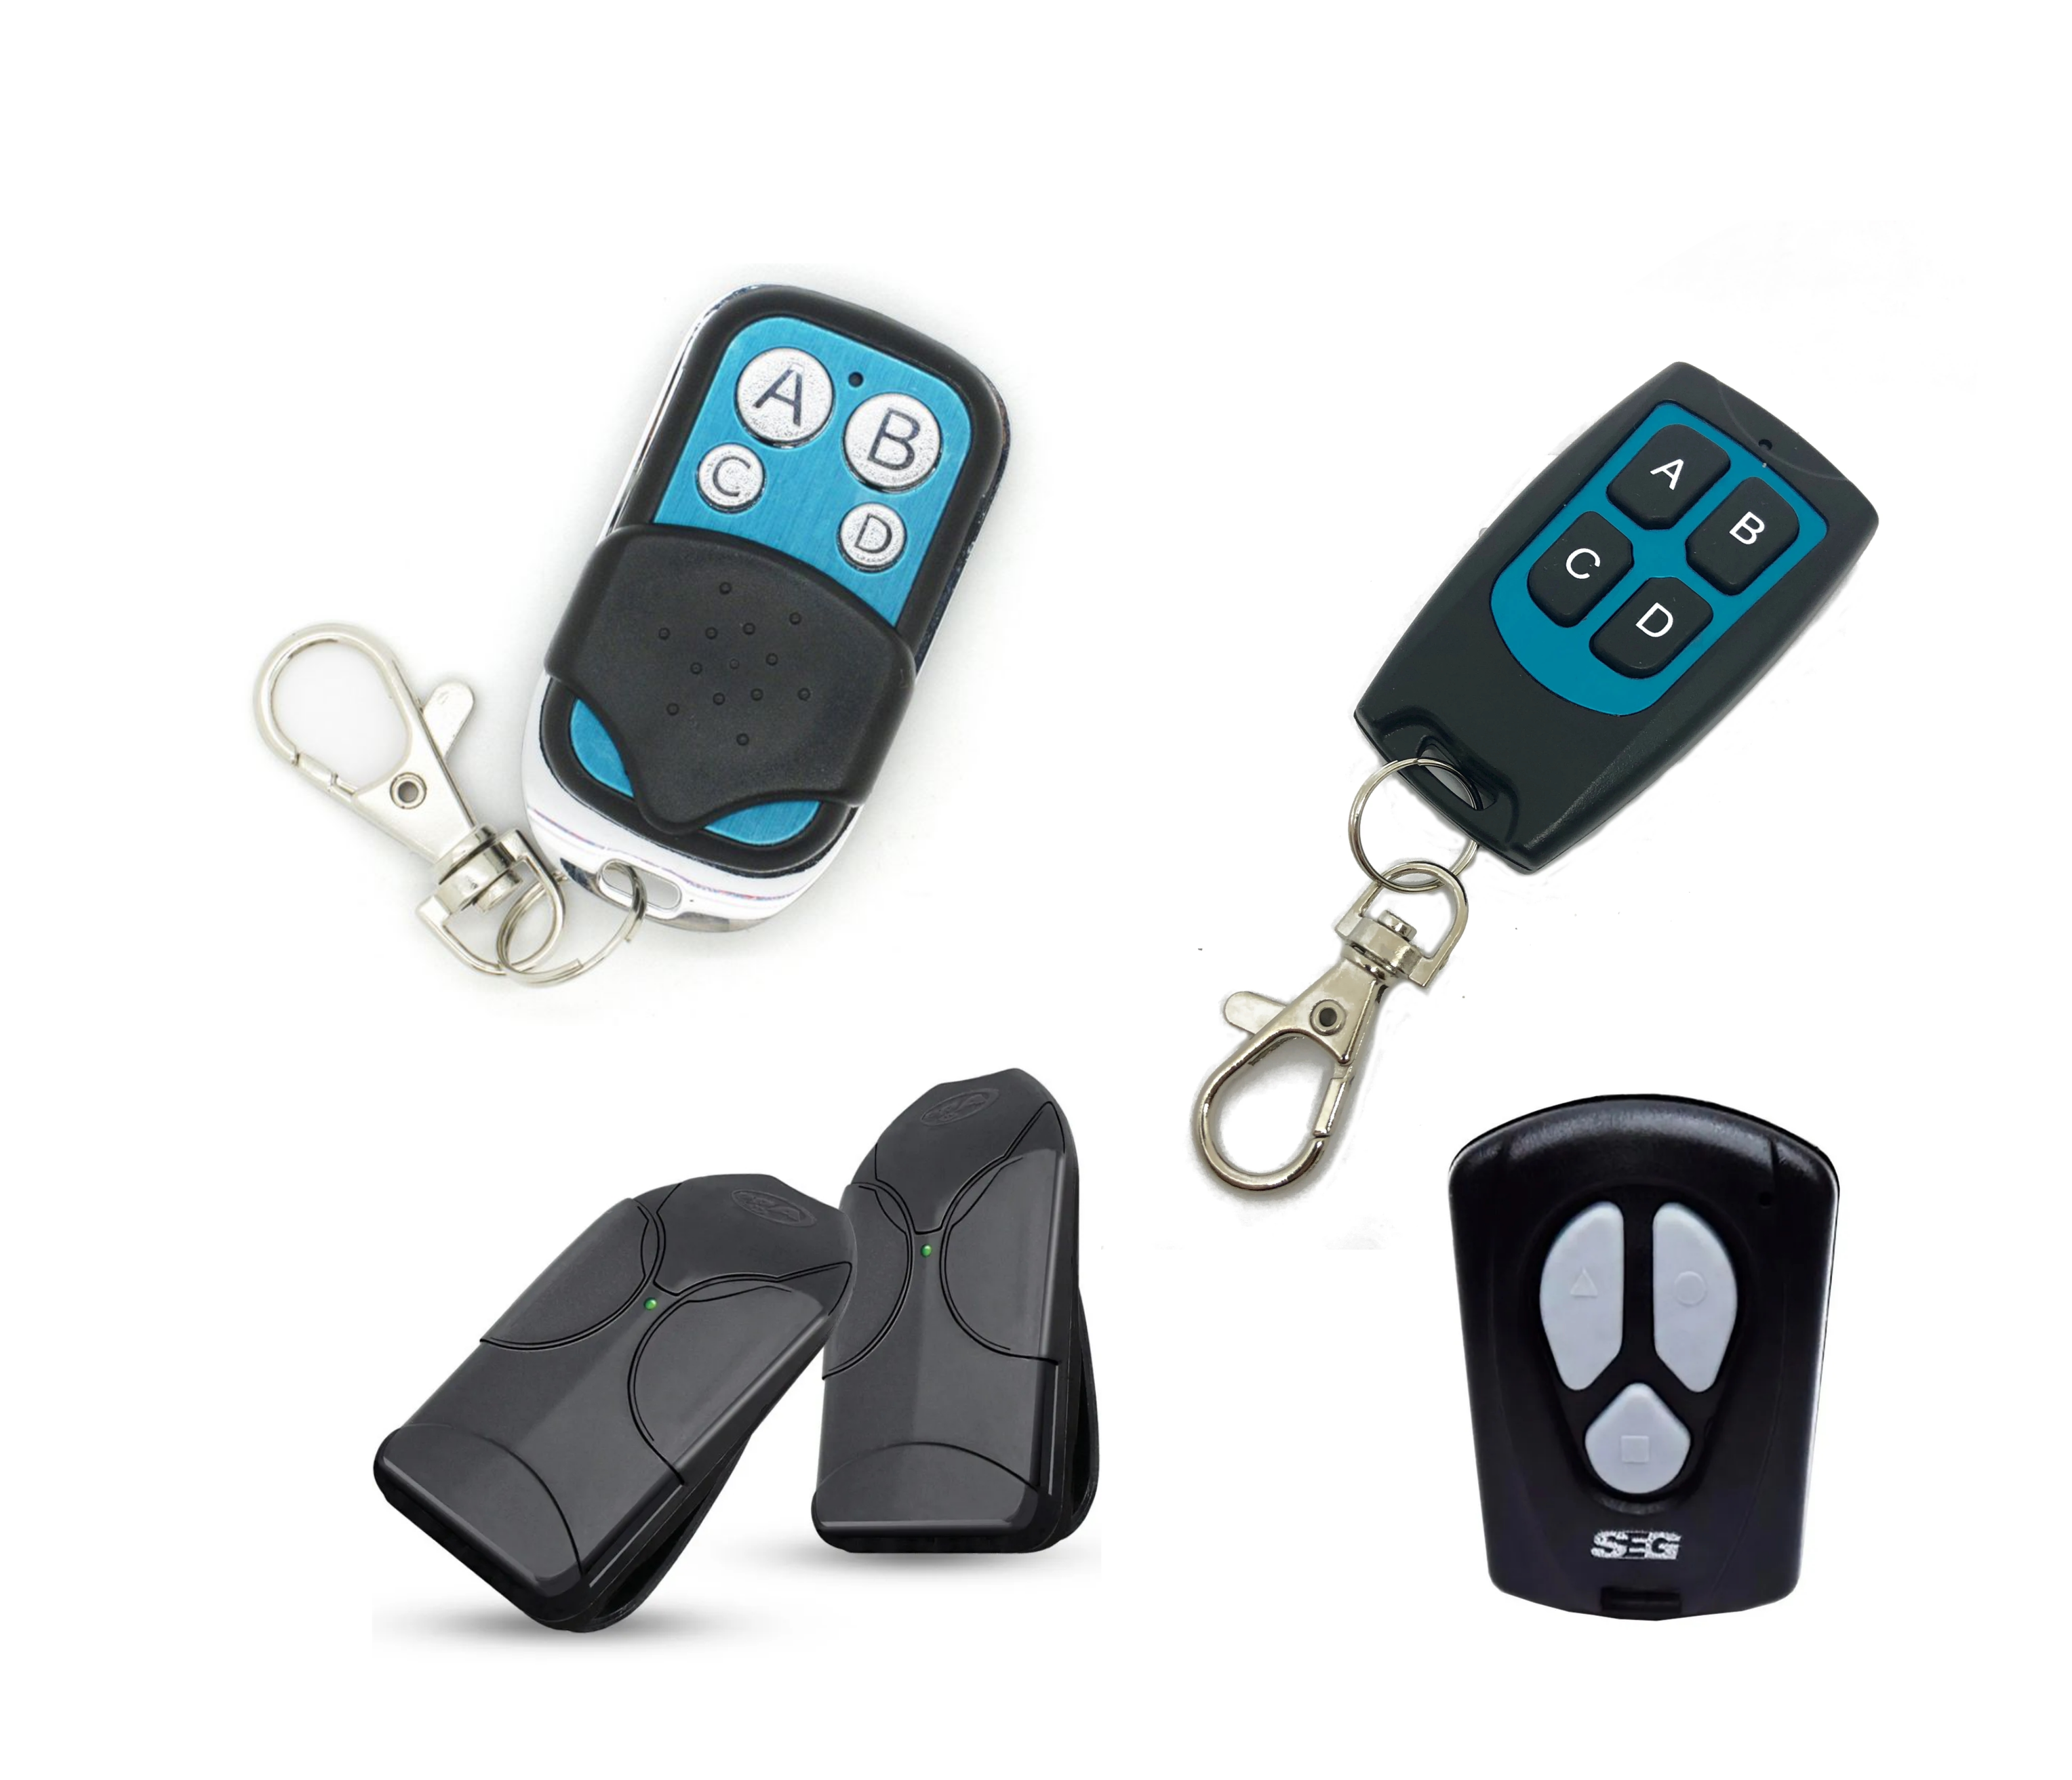
\includegraphics[width=0.6\textwidth]{Pictures/controlesrf.png}
	\rule{35em}{1pt}
	\caption[Controles RF]{Controles remotos RF en diferentes presentaciones. }
	\label{fig:controlesrf}
\end{figure}

\subsubsection{Un problema de seguridad}
Tanto el empleo de llaves RFID como controles RF presentan un problema de seguridad para estos sistemas de acceso electrónico ya que conceden acceso a quien porta llave sin importar si se trata del dueño real.
En ningún caso se utilizan protocolos para la identificación del solicitante. Así mismo tampoco se emplean algoritmos de  encripción de datos por lo que el código de identificación se transmite en texto plano, por lo menos este es el caso para la mayoría de las implementaciones.\\
Por esta razón existen métodos de hacking ya documentados que involucran dos técnicas principales.\\
\textbf{Clonado por lectura RFID:} En este caso simplemente basta con tener un lector RF y acceso a la etiqueta RFID empleada por la llave a ser clonada. Una vez leído el código se crea una etiqueta con el mismo código y se obtiene acceso.\\
\textbf{Clonado por intercepción RF:}  Ésta técnica implica un ataque por sniffing del código de identificación. Teniendo en cuenta que la frecuencia y el tipo de modulación empleado por los sistemas actuales son conocidos, resulta en una tarea sencilla empleando un transeptor RF y un decodificador por software.\\
\textbf{Inhibición de Señal:} Esta técnica es quizás la mas sencilla de todas. Se utiliza para vulnerar los sistemas de acceso que emplean controles remotos RF. Implica la utilización de un transmisor que contamina con ruido el ancho de banda de operación del control remoto. De esta forma se impide la correcta comunicación con el controlador del cerramiento al momento de enviar la señal de cierre, evitando así que la abertura pueda ser cerrada.

\section{Cerramientos Electrónicos IoT}
IoT (Internet of Things) describe la red de objetos físicos que incorporan circuitos con microcontroladores, software embebido, sensores y componentes de comunicación con el propósito de intercambiar datos con otros objetos conectados y servicios en linea a través de internet.
Teniendo en cuenta que las aberturas de un edificio son objetos físicos y que los cerramientos eléctricos ofrecen un modo de accionamiento electrónico para estos objetos, es posible concebir la adaptación de los mismos para convertirlos en implementaciones IoT.
Con el ánimo de ilustrar el panorama de productos IoT orientados a la seguridad y al control de acceso se mencionan las categorías más relevantes.

\begin{itemize}
	\item Smart Alarms
	\item Smart Door Locks
	\item Smart Garage Doors
\end{itemize}

\subsection{Smart Alarms}
Estos productos proponen la instalación y configuración de una red de sensores (comúnmente inalámbricos) en el interior y alrededor del hogar o cualquier edificio en general. Algunos ejemplos de estos sensores se listan a continuación:
\begin{itemize}
	\item Sensores de Humo
	\item Sensores de gases peligrosos (CO2, CO, propano, butano, metano).
	\item Sensores de presencia IR.
	\item Sensores de apertura para puertas y ventanas.
\end{itemize} 
Estos sensores son sistemas embebidos de tamaño reducido con poca capacidad de cómputo y de muy bajo consumo eléctrico incluso en algunas versiones alimentados a baterías.
Por esta razón se emplean protocolos de comunicación acorde a las capacidades de estos dispositivos tales como \textit{zigbee} y \textit{Thread} ambos basados en la especificación IEEE 802.15.4 por lo que sus respectivos stacks de software presentan footprints de memoria adecuados para la aplicación en particular.\\
Como parte fundamental de la red se incluye un dispositivo electrónico denominado \textit{concentrador, gateway ó central} que posee al menos dos interfaces de comunicación principales, una para conectarse a la red de sensores y otra para acceder a internet. Este ''gateway'' recibe las actualizaciones de estado de los sensores y las reenvía por internet a un servicio de monitoreo mantenido por el mismo proveedor.\\
El usuario puede acceder a los datos almacenados por el servicio a través de un cliente web o aplicación móvil.
Adicionalmente estos clientes ofrecen una GUI para la configuración tanto de la central como para los sensores.
En la figura ~\ref{fig:smartalarms} se muestran ejemplos de los productos ofrecidos por los fabricantes más populares.

\begin{figure}[htbp]
	\centering
	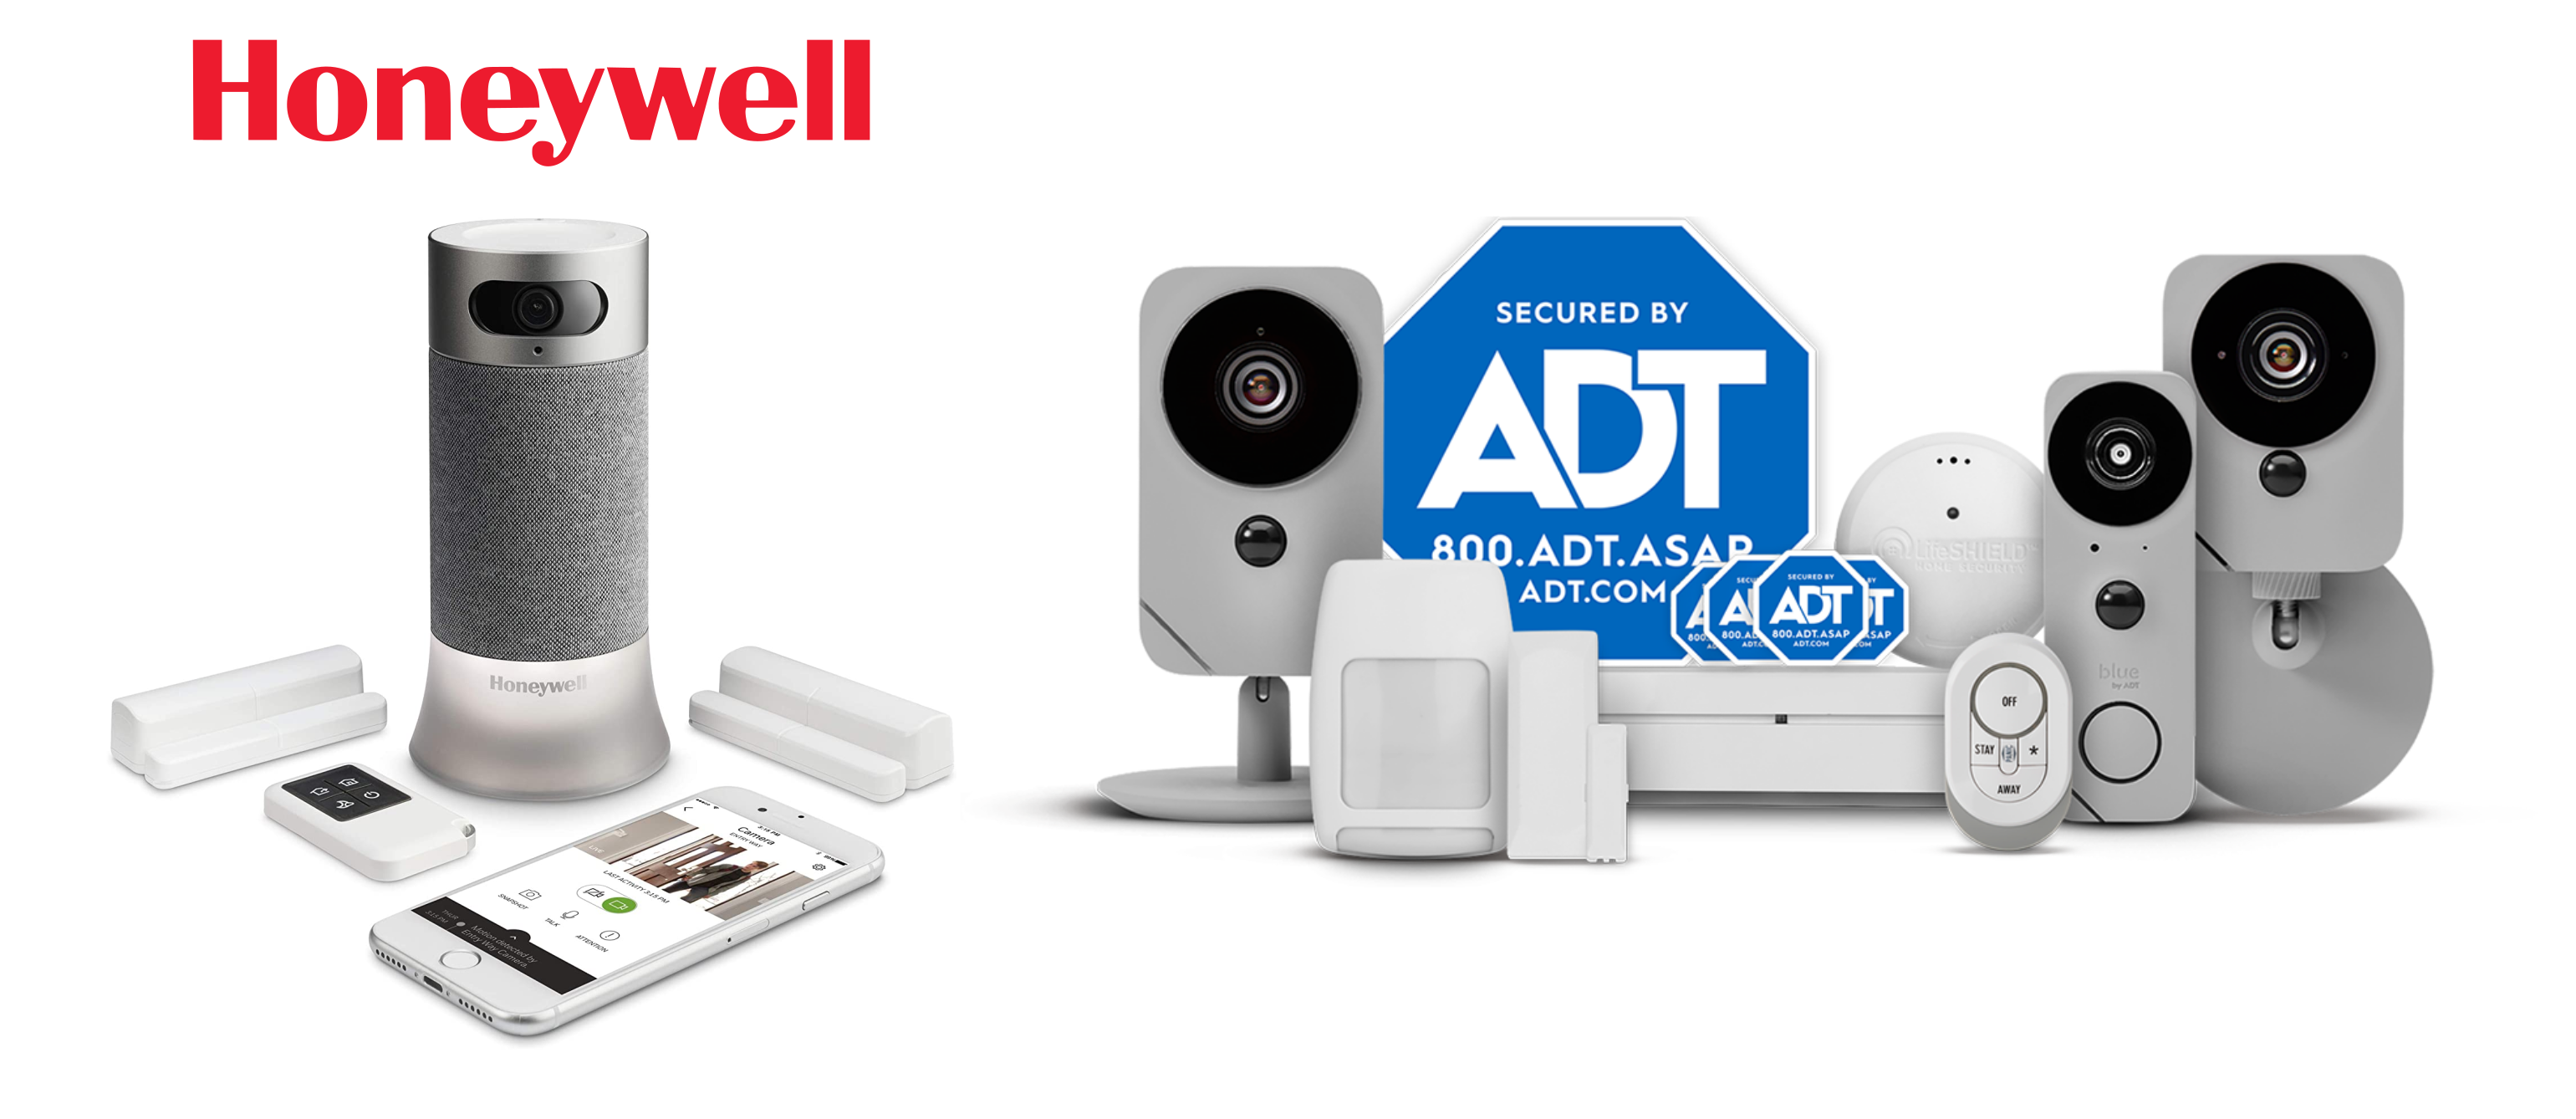
\includegraphics[width=0.8\textwidth]{Pictures/smartalarms.png}
	\rule{35em}{1pt}
	\caption[Smart Alarms]{Familia de productos de los fabricantes mas conocidos.}
	\label{fig:smartalarms}
\end{figure}

\subsection{Smart Door Locks}
Esta categoría de productos comprenden dispositivos electromecánicos que reemplazan o se adaptan a las tradicionales cerraduras de tambor radial comúnmente utilizadas en puertas residenciales estadounidenses.
Estos dispositivos incluyen el sistema embebido capaz de conectarse a internet a través de WiFi o Bluetooth (mediante el uso de un gateway WiFi como en el caso de SESAME).
Para todos los casos se ofrece una aplicación móvil que hace de llave virtual y permite el acceso a estos cerramientos inteligentes.
Adicionalmente el usuario administrador podrá agregar y remover usuarios autorizados a operar el dispositivo.
En la figura ~\ref{fig:smartlocks} se pueden observar ejemplos reales de productos disponibles en el mercado.

\begin{figure}[htbp]
	\centering
	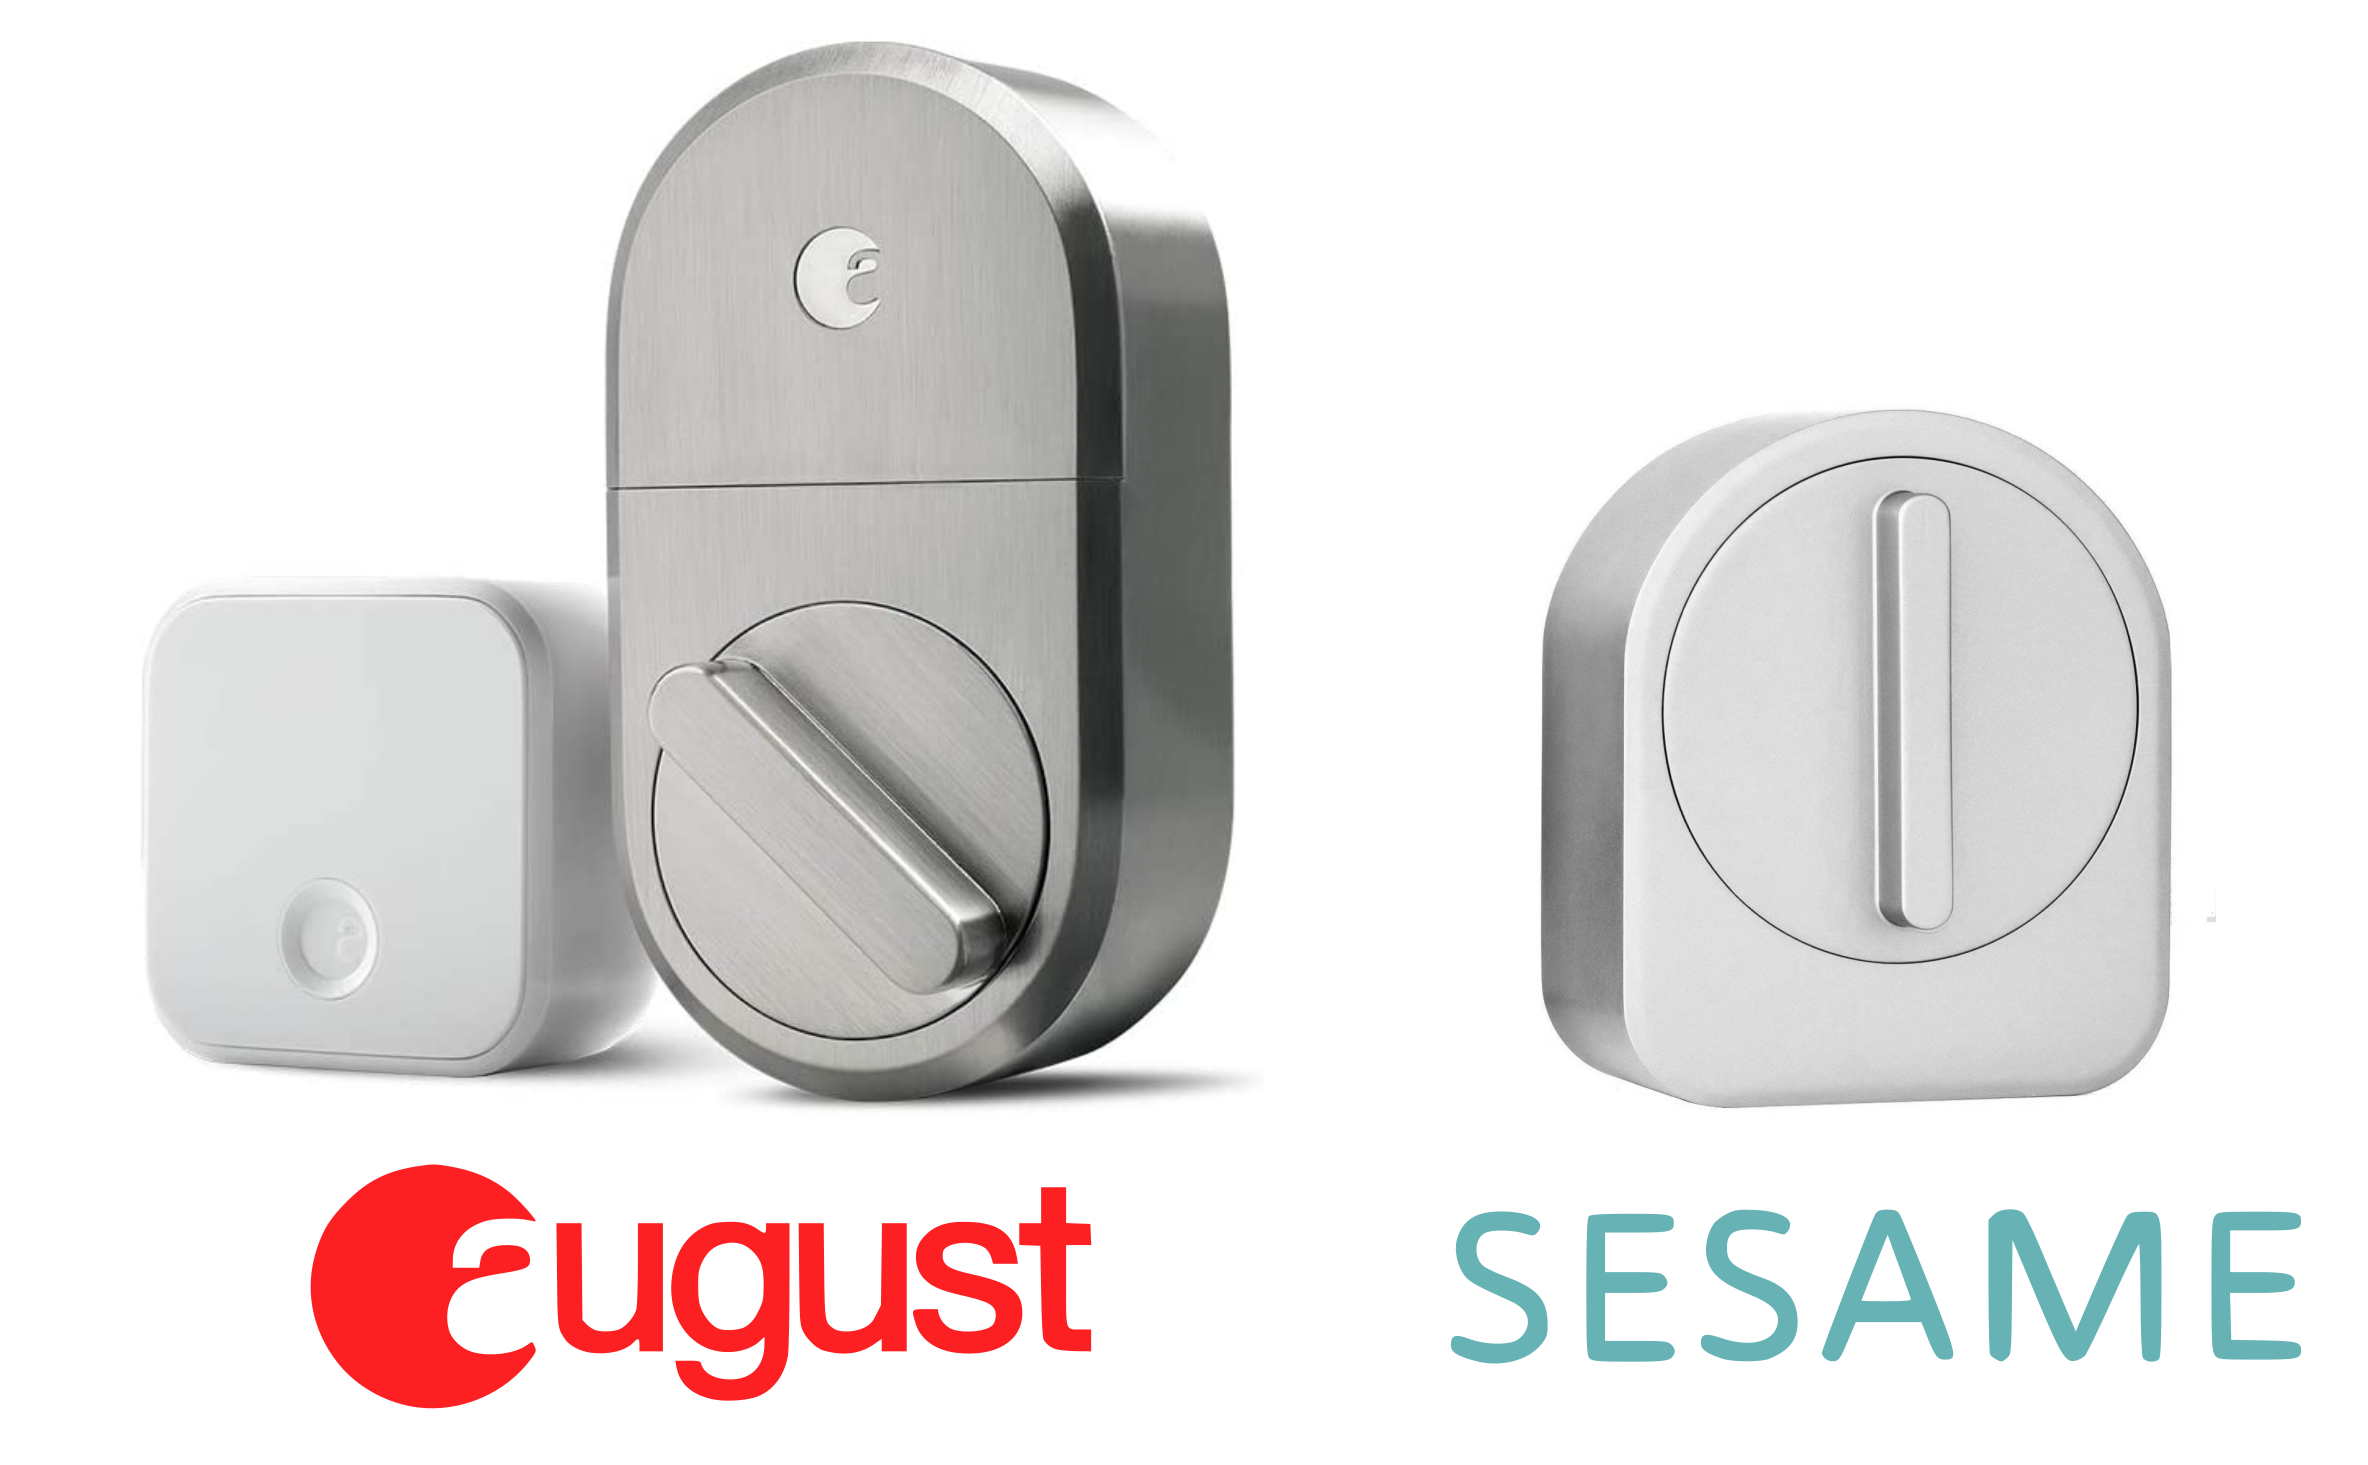
\includegraphics[width=0.6\textwidth]{Pictures/smartlocks.png}
	\rule{35em}{1pt}
	\caption[Smart Locks]{Modelos más comercializados de cerraduras inteligentes.}
	\label{fig:smartlocks}
\end{figure}

\subsection{Smart Garage Door}
Para el caso de los portones automatizados de garaje existen diversas implementaciones que agregan estos objetos a la familia de productos IoT.\\
La mayoría de los controladores ofrecen al menos una interfaz para conexión de un botón externo de apertura y cierre. Por esta razón diversas sturtups desarrollaron implementaciones de dispositivos a modo de accesorios compatibles con una familia de controladores. Este es el caso de ISmartGate, Nexx NXG-100 y Garadget.\\
Luego los fabricantes más importantes de controladores y motores para portones de garaje de estados unidos realizaron sus propias implementaciones y las incorporaron a sus controladores como una funcionalidad built-in. Este es el caso de la empresa Genie con su linea de productos Aladdin. Por otro lado la empresa Chamberlane optó por el enfoque de agregar la misma funcionalidad mediante el uso de accesorios que ofrecen con su línea myQ.\\
Mas recientemente, en el transcurso del año 2019 PPA, la empresa más grande de Sudamérica especializada en automatización de aberturas residenciales e industriales. Presentó un gateway IoT (SPIRIT) compatible con una amplia familia de sensores y actuadores que también fabrican. Entre ellos un módulo que permite el accionamiento y monitoreo remoto de portones automatizados.
Todas las implementaciones ofrecen una aplicación móvil que se usará para el monitoreo, control y configuración del producto.
En la figura ~\ref{fig:smartgates} se muestran ejemplos de estos productos.

\begin{figure}[htbp]
	\centering
	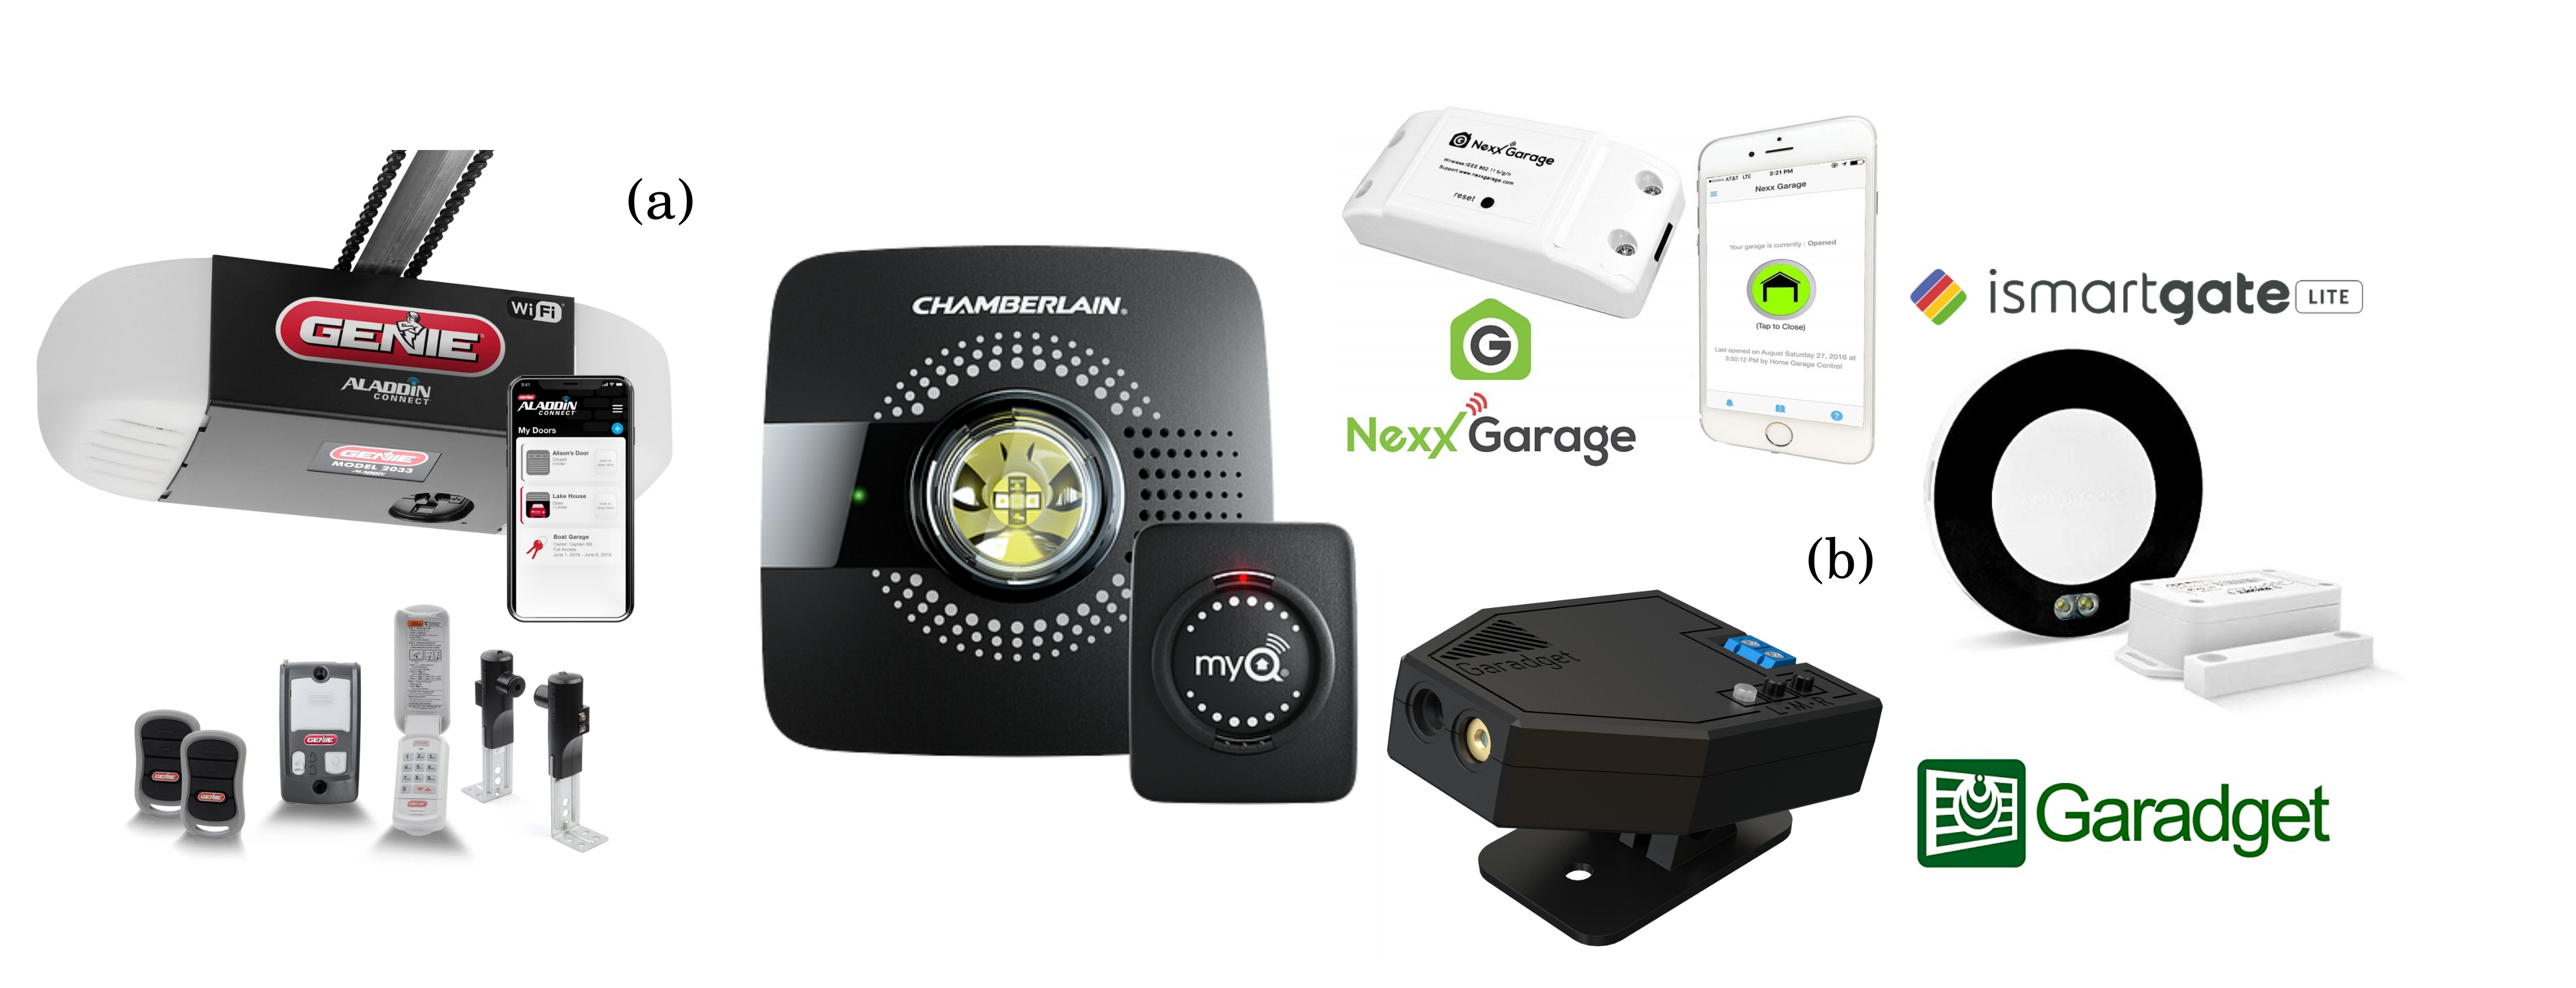
\includegraphics[width=0.8\textwidth]{Pictures/smartgates.png}
	\rule{35em}{1pt}
	\caption[Smart Garage Gates]{Modelos más comercializados de automatización inteligente para portones de garaje.}
	\label{fig:smartgates}
\end{figure}

\section{Conclusión}
Los cerramientos eléctricos presentan una interesante gama de dispositivos para los que pueden plantearse la extensión de funcionalidad con el objetivo de convertirlos en productos IoT. Algunas de las funcionalidades que se entienden deseables para este tipo de dispositivos son el monitoreo remoto, el control a distancia y la configuración remota.\\
Adicionalmente aparece una oportunidad de mejora al plantear los problemas de seguridad que tienen las implementaciones actuales y que podrían ser mitigados al utilizar protocolos de comunicación modernos.
